\ifdefined\JOURNAL

In this section, we introduce the LVars programming model, first with
a motivating problem and a series of brief code examples, and then
with $\lambdaLVar$, a deterministic parallel calculus with shared
state that extends the call-by-value $\lambda$-calculus with a store
and @put@ and @get@ operations.  The main technical result of
this \either{chapter}{section} is a proof of determinism for
$\lambdaLVar$ (Section~\ref{s:lvars-proof}).  Finally, we consider a
more expressive semantics for the @put@ operation that generalizes
from least-upper-bound writes to arbitrary inflationary, commutative
writes.

\fi

\ifdefined\DISSERTATION

Programs written using a \emph{deterministic-by-construction} model of
parallel computation are guaranteed to always produce the same
observable results, offering programmers freedom from subtle,
hard-to-reproduce nondeterministic bugs.  While a number of popular
languages and language extensions (\eg, Cilk~\cite{cilk}\lk{Any
  others?}) \emph{encourage} deterministic parallel programming, few
of them guarantee determinism at the language level---that is, for
\emph{all} programs that can be written using the model.

Of the options available for parallel programming with a
language-level determinism guarantee, perhaps the most mature and
broadly available choice is pure functional programming with
function-level task parallelism, or \emph{futures}.  For example,
Haskell programs using futures by means of the @par@ and @pseq@
combinators can provide real speedups on practical programs while
guaranteeing determinism~\cite{marlow-par}.\footnote{When programming
  with \lstinline|par| and \lstinline|pseq|, a language-level
  determinism guarantee obtains if user programs are written in the
  \emph{Safe Haskell}~\cite{safe-haskell} subset of Haskell (which is
  implemented in GHC Haskell by means of the \lstinline|SafeHaskell|
  language pragma), and if they do not use the \lstinline|IO| monad.}
Yet pure programming with futures is not ideal for all problems.
Consider a \emph{producer/consumer} computation in which producers and
consumers can be scheduled onto separate processors, each able to keep
their working sets in cache.  Such a scenario enables \emph{pipeline
  parallelism} and is common, for instance, in stream processing.  But
a clear separation of producers and consumers is difficult with
futures, because whenever a consumer forces a future, if the future is
not yet available, the consumer immediately switches roles to begin
computing the value (as explored by Marlow \etal~\cite{monad-par}).

Since pure programming with futures is a poor fit for
producer/consumer computations, one might then turn to \emph{stateful}
deterministic parallel models.  Shared state between computations
allows the possibility for race conditions that introduce
nondeterminism, so any parallel programming model that hopes to
guarantee determinism must do something to tame sharing---that is, to
restrict access to mutable state shared among concurrent computations.
Systems such as Deterministic Parallel Java~\cite{dpj-oopsla,
  dpj-hotpar09}, for instance, accomplish this by ensuring that the
state accessed by concurrent threads is \emph{disjoint}.
Alternatively, a programming model might allow \emph{data} to be
shared, but limit the \emph{operations} that can be performed on it to
only those operations that commute with one another and thus can
tolerate nondeterministic thread interleavings.  In such a setting,
although the order in which side-effecting operations occur can differ
on multiple runs, a program will always produce the same observable
result.\footnote{There are many ways to define what is observable
  about a program. As noted in \either{Chapter}{Section}~\ref{ch:intro}, \either{I}{we} define the
  observable behavior of a program to be the value to which it
  evaluates.}

\ifdefined\DISSERTATION
\begin{wrapfigure}{l}{2.7in}
\vspace{-1em}
\begin{center}
  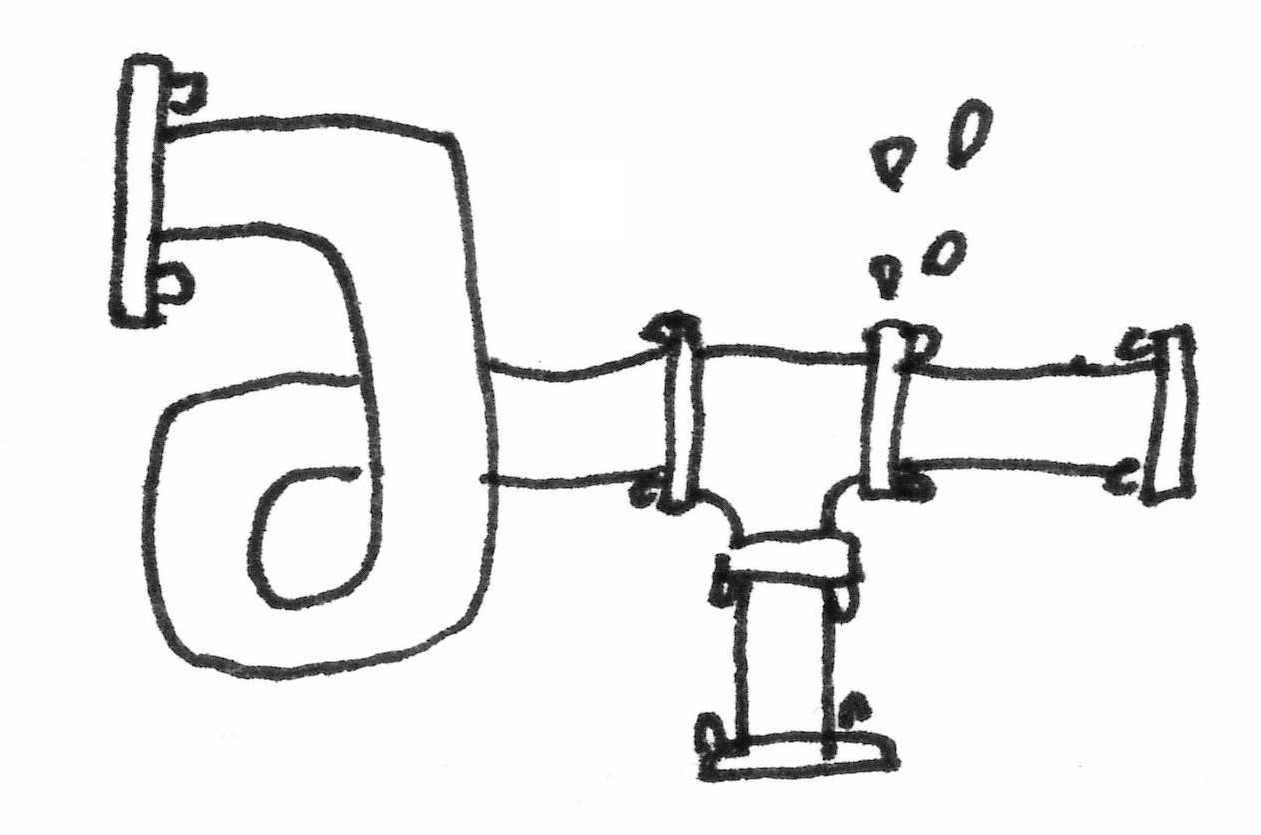
\includegraphics[scale=0.15]{../illustrations/flow3}
\end{center}
\vspace{-1em}
\end{wrapfigure}
\fi

In Kahn process networks (KPNs)~\cite{Kahn-1974} and other
\emph{data-flow parallel} models---which are the basis for
deterministic stream-processing languages such as
StreamIt~\cite{streamit-asplos}---communication among processes takes
place over blocking FIFO queues with ever-increasing \emph{channel
  histories}.  Meanwhile, in
\emph{single-assignment}~\cite{Tesler-1968} or
\emph{IVar-based}~\cite{IStructures} programming models, such as the
Intel Concurrent Collections system (CnC)~\cite{CnC} and the
\emph{monad-par} Haskell library~\cite{monad-par}, a shared data store
of blocking single-assignment memory locations grows monotonically.
Hence both programming models rely on \emph{monotonic data
structures}: data structures to which information can only be added
and never removed, and for which the timing of updates is not
observable.

Because state modifications that only add information and never
destroy it can be structured to commute with one another and thereby
avoid race conditions, it stands to reason that diverse deterministic
parallel programming models would leverage the principle of
monotonicity.  Yet systems like StreamIt, CnC, and monad-par emerge
independently, without recognition of their common basis.  Moreover,
since each one of these programming models is based on a single type
of shared data structure, they lack \emph{generality}: IVars or FIFO
streams alone cannot support all producer/consumer applications, as \either{I}{we}
discuss in Section~\ref{s:lvars-motivation}.

Instead of limiting ourselves to a single type of shared data
structure, though, we can take the more general notion of monotonic
data structures as the basis for a new deterministic parallel
programming model.  In this \either{chapter, I}{section, we} show how to generalize IVars
to \emph{LVars}, thus named because the states an LVar can take on are
elements of a given \emph{lattice}.\footnote{This
``lattice'' need only be a \emph{bounded join-semilattice} augmented
with a greatest element $\top$, in which every two elements have a
least upper bound but not necessarily a greatest lower bound; see
Section~\ref{subsection:lvars-lattices}.  For brevity, \either{I}{we} use the term
``lattice'' in place of ``bounded join-semilattice with a designated
greatest element'' throughout this dissertation.}  This lattice determines the semantics of the @put@ and
@get@ operations that comprise the interface to LVars (which \either{I}{we} will
explain in detail in \either{the sections that follow}{the rest of this section}): the @put@ operation
takes the least upper bound of the current state and the new state
with respect to the lattice, and the @get@ operation performs
a \emph{threshold read} that blocks until a lower bound in the lattice
is reached.

Section~\ref{s:lvars-examples} introduces the concept of LVars through
a series of small code examples.  Then, in Sections~\ref{s:lvars-lattices}
and~\ref{s:lvars-lambdalvar} \either{I}{we} formally define $\lambdaLVar$, a
deterministic parallel calculus with shared state, based on the
call-by-value $\lambda$-calculus.  The $\lambdaLVar$ language is
general enough to subsume existing deterministic parallel languages
because it is parameterized by the choice of lattice.  For example, a
lattice of channel histories with a prefix ordering allows LVars to
represent FIFO channels that implement a Kahn process network, whereas
instantiating $\lambdaLVar$ with a lattice with one ``empty'' state
and multiple ``full'' states (where $\forall{i}.\; \mathit{empty}
< \mathit{full_i}$) results in a parallel single-assignment language.
Different instantiations of the lattice result in a family of
deterministic parallel languages.

Because lattices are composable, any number of diverse monotonic data
structures can be used together safely.  Moreover, as long as a data
structure presents the LVar interface, it is fine to wrap an existing,
optimized concurrent data structure implementation; we need not
rewrite the world's data structures to leverage the $\lambdaLVar$
determinism result.

The main technical result of this \either{chapter}{section} is a proof of determinism
for $\lambdaLVar$ (Section~\ref{s:lvars-proof}).  The key lemma,
Independence (Section~\ref{subsection:lvars-independence}), gives a
kind of \emph{frame property} that captures the commutative effects of
LVar computations.  Such a property would \emph{not} hold in a typical
language with shared mutable state, but holds in the setting of
$\lambdaLVar$ because of the semantics of @put@ and @get@.

Finally, in Section~\ref{s:lvars-generalizing}, \either{I}{we} consider some
alternative semantics for the @put@ and @get@ operations that
generalize their behavior while retaining the determinism of the
original semantics: \either{I}{we} generalize the @put@ operation from
least-upper-bound writes to inflationary, commutative writes, and \either{I}{we}
generalize the @get@ operation to allow a more general form of
threshold reads.
\fi
